%%%%%%%%%%%%%%%%%%%%%%%%%%%%%%%%%%%%%%%%%%%%%%%%%%%%%%%%%%%%%%%%%%%%%%%%%%%%%%%%
% Diese Datei beinhaltet den eigentlichen Inhalt Ihrer Arbeit.
%
% Es bietet sich der Übersicht halber an, die einzelnen Abschnitte jeweils
% in eigene Dateien zu schreiben und mittels \input einzubinden.
% Eine mögliche Verzeichnisstruktur sähe entsprechend so aus:
%
%     thesis/
%     +- tex/
%     |  +- introduction.tex
%     |  +- motivation.tex
%     |  +- experiments.tex
%     |  |  ...
%     |  +- conclusion.tex
%     +- abstract.tex
%     +- contents.tex
%     +- thesis.tex
%%%%%%%%%%%%%%%%%%%%%%%%%%%%%%%%%%%%%%%%%%%%%%%%%%%%%%%%%%%%%%%%%%%%%%%%%%%%%%%%

\section {Generelles und Technologien}

\subsection{WebAssembly}

\begin{itemize}
  \item binäres Instruktionsformat für stack basierte VM
  \item effizienter als JS
  \item kein ersatz für JS als Ganzes, sondern nur für rechenintensive teile
  \item compilation target für viele Programmiersprachen wie C/C++ oder Rust
\end{itemize}

WebAssembly (Wasm) ist ein binäres Instruktionsformat für eine Stack-basierte virtuelle Maschine welche in allen modernen Browsern enthalten ist.
Dieses Instruktionsformat wird von verschiedenen Programmiersprachen als kompilierungs Zielsprache genutzt um eine effizientere Alternative zu JavaScript(JS) für die Browserprogrammierung zu bieten.
Wasm ist jedoch kein Ersatz für JavaScript und hat somit keinen direkten Zugriff auf den DOM oder Events, sondern dient dazu besonders rechenintensive Funktionen in einer sonst nativen Programmiersprache wie C/C++ oder Rust zu schreiben.

\subsection{Rust}

\begin{itemize}
  \item Multiparadigmen-Systemprogrammiersprache
  \item Systemprogrammierung sicher und zugänglicher machen
  \item kann zu wasm compilen
  \item kein GC, aber trotzdem automatische Speicherbereinigung zur Compile time
  \item starkes, statisches typsystem inspiert von ML und Haskell
\end{itemize}

Rust ist eine Multiparadigmen-Systemprogrammiersprache welche entwickelt wurde um Systemprogrammierung sicherer und zugänglicher zu machen. Neben der Option zu nativen Maschinencode zu kompilieren, bietet Rust auch die Option Wasm als Zielplattform zu verwenden und kann somit für Browserprogrammierung verwendet werden.
Genau wie C/C++ hat Rust keine Gargabe Collection zur Laufzeit, sondern verlässt sich auf explizite Funktionsaufrufe um Speicher freizugeben, jedoch muss der Programmierer diese Aufrufe nicht selber programmieren, anders als in C oder C++, deren Speichermodell generell als umständlich und fehleranfällig gilt.
Stattdessen fügt der Compiler alle benötigten Aufrufe selbständig ein. Dies ermöglicht Rust die besten Eigenschaften beider Welten zu vereinen. Speicherverwaltung hat keine zusätzlichen Laufzeitkosten, ist aber trotzdem voll automatisch.
Natürlich hat aber auch dieser Ansatz Nachteile. Um es dem Rust Compiler zu ermöglichen allen benutzen Speicher an der korrekten Stelle freizugeben, muss der Programmierer einige Regeln einhalten. Zuweilen werden an manchen Stellen explizite Angaben über die Lebensdauer von Referenzen benötigt, was Rust Code teils aufwendig zu schreiben macht.
Eine weitere wichtige Eigenschaft von Rust ist das sehr starke, von ML und Haskell inspierte, Typsystem, welches es dem Programmierer ermöglicht komplexe Einschränkungen und Möglichkeiten für Typen festzulegen.

\subsection{Die Vorteile von Rust gegenüber JavaScript}

\begin{itemize}
  \item Performance
  \item Stabilität und Zuverlässigkeit durch starkes, statisches Typsystem
  \item Nützliche Sprach features wie: Enums, Pattern Matching und Traits
  \item Gutes tooling: Cargo zum Bauen und Testen in Einem
\end{itemize}

\subsection{Die Vorteile von Rust gegenüber anderen Wasm-Sprachen}

\begin{itemize}
  \item Performance und Bundle size (kein GC, kleine Runtime)
  \item stabiles Ökosystem: wasm-bindgen, web-sys, console\_error\_panic\_hook
  \item stabile Sprache mit gutem Editor support (im Vergleich zu Zig, Nim, ...)
  \item sicherer und praktischer als C/C++
\end{itemize}

\subsection{React.js}

\begin{itemize}
  \item Industrie Vorreiter für dynamische Frontend Entwicklung
  \item Sehr stabil und mature, mit unzähligen resourcen
\end{itemize}

\subsection{Die Vorteile von React.js gegenüber rohem JavaScript}

\begin{itemize}
  \item Componenten architektur vereinfacht Code re-use stark
  \item Einfache, deklarative und effiziente updates für Components
  \item UI = f(state) anstatt imperativer spagetti code
\end{itemize}

\section{Abgrenzungen zu Fremdleistungen}

\subsection{Nand to Tetris}
\begin{itemize}
  \item VM Bytecode design und high level Funktionalität
  \item CPU Assembly design und high level Funktionalität
  \item TST design und high level Funktionalität
  \item Viele Tests für Emulatoren aus N2T Projekten
\end{itemize}

\subsection{Dependencies}
\begin{itemize}
\item lazy\_static (hack um rust weniger nervig zu machen)
\item regex
\item wasm-bindgen (rust code für JS zugänglich machen)
\item web-sys (js stdlib in Rust nutzen)
\item console\_error\_panic\_hook (rust panics zu JS exeptions)
\item sdl2 (native UI (eigentlich nur zum Testen))
\item clap (CLI parsing)
\item wasm-pack (rust -> wasm Kompilierung einfacher machen)
\item react und npm (UI)
\end{itemize}

\subsection{Related Work}
\begin{itemize}
  \item https://github.com/itoshkov/nand2tetris-emu
  \item https://github.com/mossprescott/pynand
\end{itemize}

\section{Nand to Tetris and the Hack Architecture}

Nand to Tetris is divided into several sections that can be worked on or skipped more or less independently of each other.
Each section is further removed from the actual hardware than its predecessor. In the beginning, the students create the necessary chips and logic gates, starting with only a nand gate. This section is not part of this thesis at all, but it may be relevant in future additions to the application~\ref{future-work}.
After that, the students will work with assembly language and create an assembler of their own, the generated code of which will target the CPU from the previous section.
The application created as part of this thesis includes an emulator, that is able to run the assembly directly without any further compilation. This allows students to run their assembly code in the same application as their VM code from the later sections.
In the next section, students will work closely with VM bytecode, first by writing a translator from bytecode to assembly, and later by writing a complete game using the high-level programming language that will be implemented in the last section.
In the end, students will create a compiler for a high-level language called Jack, that is part of the course. They will also implement a standard library for this language, that abstracts many of the direct interactions with the platform, such as printing text to the screen.
The last two parts are relevant to this project because students can run both the VM code and their compiled assembly inside the emulator. Furthermore, the main focus of this project is the aforementioned game that is created in Project 9.
It may seem strange to develop a whole new emulator mainly to improve a single one of twelve projects, but that single project is the ``Tetris'' to which the title of the course refers. Even though Project 9 is not the last project, it is still the highlight of the course for many people.
This is illustrated by the fact that nine of the twelve examples listed under the ``Cool Stuff''~\cite{n2tweb} tab on the official website are Jack programs that would qualify as Project 9 solutions.
Therefore, if your goal is to improve the overall student experience, it makes sense to focus on this project in particular.
Despite that, this the emulators created as part of this project may also improve the experience for other projects.~\ref{evaluation}

% \subsection{The sections of Nand to Tetris}
% \begin{itemize}
%   \item Chips und Logic Gates (nicht Teil der Arbeit)
%   \item CPU und Assembly
%   \item Virtuelle Machine
%   \item High level Sprache und Betriebssystem (nicht Teil der Arbeit)
% \end{itemize}

\subsection{How does the Hack VM work}
\subsubsection{Example: Adding numbers in a Loop}
\begin{lstlisting}[language=C, caption={Calculate 1 + 2 + 3 in C}, captionpos=b]
  int i = 1;
  int sum = 0;
  while (i <= 3) {
    sum += i;
    i++;
  }
\end{lstlisting}

explain push/pop in detail
explain how the stack works

\subsection{Hack Bytecode} \label{hack-bytecode}
\begin{lstlisting}[caption={Calculate 1 + 2 + 3 in the Hack VM}, captionpos=b]
  // i = 1
  push constant 1
  pop local 0

  // sum = 0
  push constant 0
  pop local 1

  label LOOP_START

  // the Hack bytecode does not have an <= instruction,
  // therefore use i < 4 instead of i <= 3
  push local 0
  push constant 4
  lt

  // if i >= 4 jump out of the loop
  not
  if-goto LOOP_END

  // sum = sum + i
  push local 1
  push local 0
  add
  pop local 1

  // i = i + 1
  push local 0
  push constant 1
  add
  pop local 0

  // jump to the beginning of the loop again
  goto LOOP_START
  label LOOP_END
\end{lstlisting}

\section{Implementierung}

\subsection{Generelles Vorgehen}
\subsubsection{VM basics außerhalb des Browsers test driven}
\begin{itemize}
  \item zuerst Bytecode parser, da dieser in VM Tests benutzt werden kann
  \item Grundlegende VM features (alles außer function, call, return)
  \item testing durch unit tests (Übersetzungen von VME.tst tests)
  \item restliche VM instructions
  \item stdlib zunächst nur als vm bytecode
\end{itemize}

\subsection{Architektur}
\subsection{Wie funtionieren Virtuelle Maschinen und Bytecode}
\subsection{VM Entwicklung in Rust}

\section{Ergebnisse}

\section{Future work}


\section{Bilder und Co.}

\subsection{Bilder}%
\label{sec:figures}

\begin{figure}[h]
  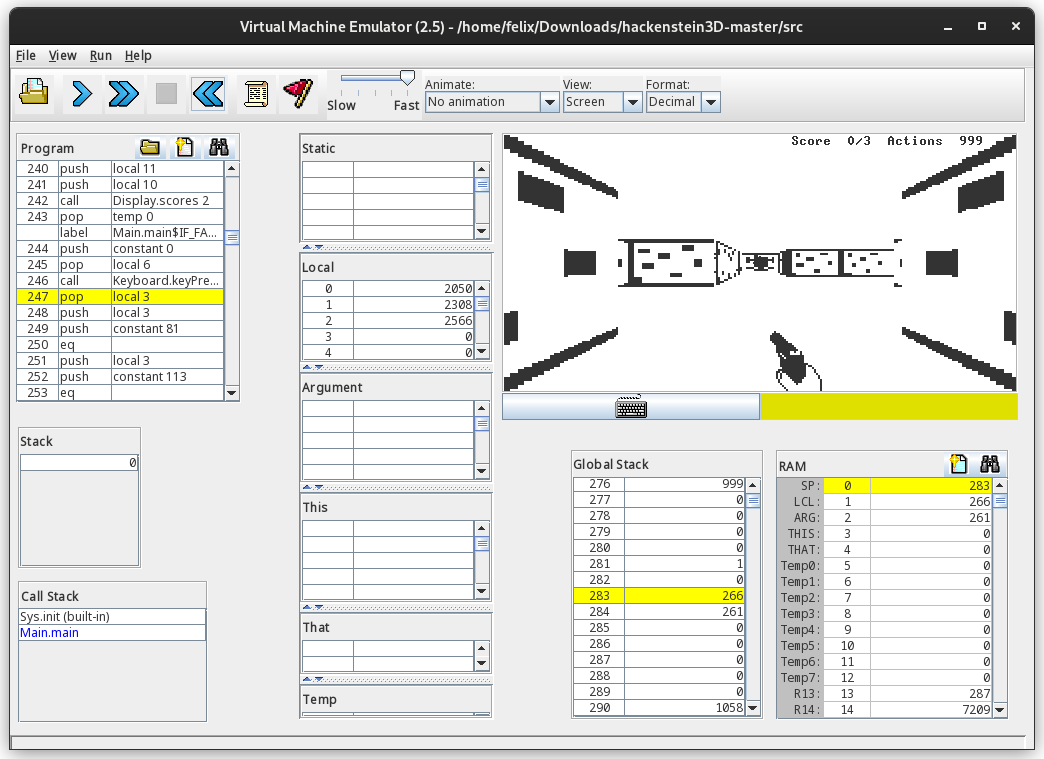
\includegraphics[width=14cm]{fig/hackenstein-offiziell.png}
  \caption{Ein simpler Wolfenstein 3D Klon im VM Emulator}%
  \label{fig:hackenstein-offiziell}
\end{figure}

\section{Fazit}

Am Ende der Arbeit werden noch einmal die erreichten Ergebnisse
zusammengefasst und diskutiert.

